\documentclass[tikz, border=8pt]{standalone}
\usepackage{tikz}
\usepackage{amsmath}
\usetikzlibrary{arrows.meta, backgrounds, calc}

\begin{document}
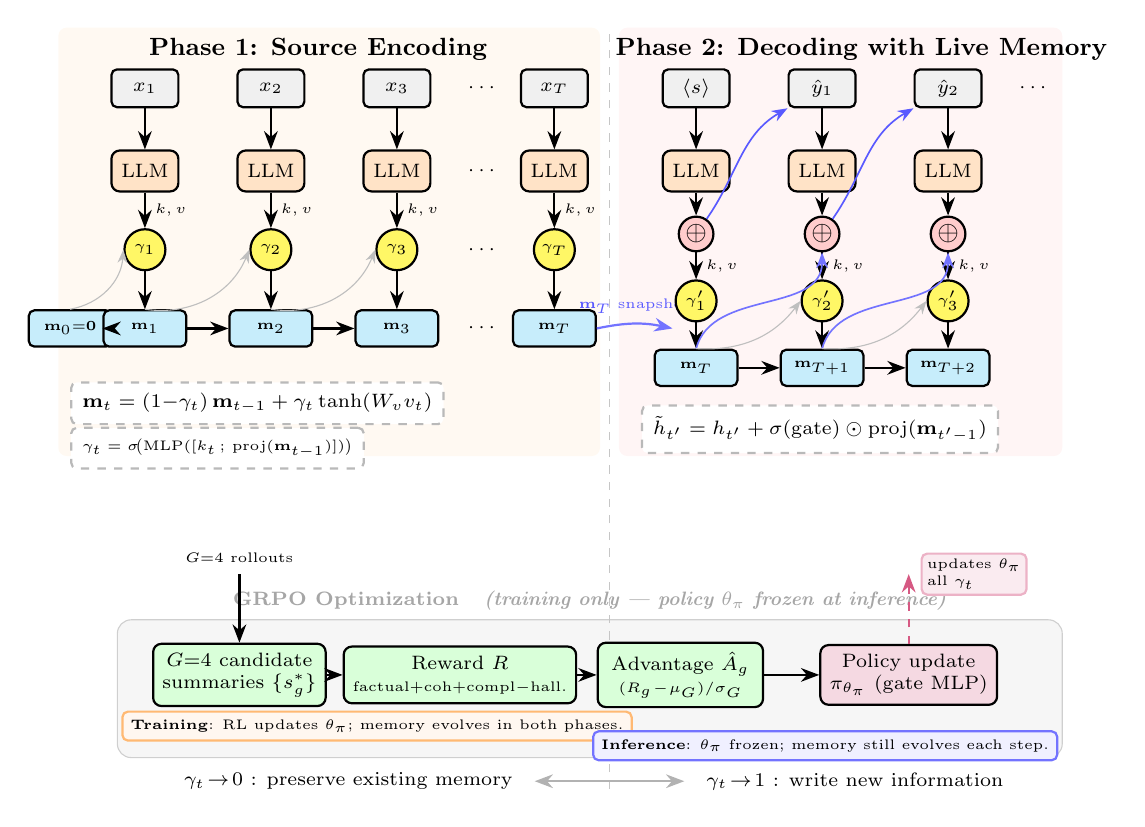
\begin{tikzpicture}[
  >=Stealth, thick,
  tok/.style  = {draw, rounded corners=2pt, fill=gray!12,
                 minimum width=0.85cm, minimum height=0.48cm, font=\scriptsize},
  llm/.style  = {draw, rounded corners=3pt, fill=orange!22,
                 minimum width=0.85cm, minimum height=0.52cm, font=\scriptsize},
  gate/.style = {draw, circle, fill=yellow!60,
                 minimum size=0.52cm, font=\tiny, inner sep=0pt},
  mem/.style  = {draw, rounded corners=2pt, fill=cyan!22,
                 minimum width=1.05cm, minimum height=0.46cm, font=\tiny},
  inj/.style  = {draw, circle, fill=red!20,
                 minimum size=0.44cm, font=\normalsize, inner sep=0pt},
  rl/.style   = {draw, rounded corners=3pt, fill=green!15,
                 minimum width=2.1cm, minimum height=0.58cm, align=center, font=\scriptsize},
  pol/.style  = {draw, rounded corners=3pt, fill=purple!15,
                 minimum width=2.1cm, minimum height=0.58cm, align=center, font=\scriptsize},
  eq/.style   = {draw=gray!55, dashed, rounded corners=2pt,
                 fill=white, inner sep=4pt, font=\scriptsize},
]

%% ── Phase labels & divider ──────────────────────────────────────────────
\node[font=\small\bfseries] at (2.2, 6.25) {Phase 1: Source Encoding};
\node[font=\small\bfseries] at (9.1, 6.25) {Phase 2: Decoding with Live Memory};
\draw[gray!45, dashed, semithick] (5.9, -3.15) -- (5.9, 6.5);

%% ── Phase 1: Tokens ─────────────────────────────────────────────────────
\node[tok] (xa) at (0.0, 5.75) {$x_1$};
\node[tok] (xb) at (1.6, 5.75) {$x_2$};
\node[tok] (xc) at (3.2, 5.75) {$x_3$};
\node[font=\scriptsize] at (4.3, 5.75) {$\cdots$};
\node[tok] (xT) at (5.2, 5.75) {$x_T$};

%% ── Phase 1: LLM ────────────────────────────────────────────────────────
\node[llm] (ha) at (0.0, 4.7) {LLM};
\node[llm] (hb) at (1.6, 4.7) {LLM};
\node[llm] (hc) at (3.2, 4.7) {LLM};
\node[font=\scriptsize] at (4.3, 4.7) {$\cdots$};
\node[llm] (hT) at (5.2, 4.7) {LLM};
\foreach \s/\t in {xa/ha, xb/hb, xc/hc, xT/hT}{\draw[->] (\s)--(\t);}

%% ── Phase 1: Gate circles ────────────────────────────────────────────────
\node[gate] (ga) at (0.0, 3.7) {$\gamma_1$};
\node[gate] (gb) at (1.6, 3.7) {$\gamma_2$};
\node[gate] (gc) at (3.2, 3.7) {$\gamma_3$};
\node[font=\scriptsize] at (4.3, 3.7) {$\cdots$};
\node[gate] (gT) at (5.2, 3.7) {$\gamma_T$};
\foreach \h/\g in {ha/ga, hb/gb, hc/gc, hT/gT}{
  \draw[->] (\h)--node[right, font=\tiny]{$k,v$}(\g);
}

%% ── Phase 1: Memory chain ────────────────────────────────────────────────
\node[mem] (m0) at (-0.95, 2.7) {$\mathbf{m}_0{=}\mathbf{0}$};
\node[mem] (m1) at ( 0.0,  2.7) {$\mathbf{m}_1$};
\node[mem] (m2) at ( 1.6,  2.7) {$\mathbf{m}_2$};
\node[mem] (m3) at ( 3.2,  2.7) {$\mathbf{m}_3$};
\node[font=\scriptsize] at (4.3, 2.7) {$\cdots$};
\node[mem] (mT) at ( 5.2,  2.7) {$\mathbf{m}_T$};

\foreach \g/\m in {ga/m1, gb/m2, gc/m3, gT/mT}{\draw[->] (\g)--(\m);}
\foreach \a/\b in {m0/m1, m1/m2, m2/m3}{\draw[->] (\a)--(\b);}

%% memory-conditioned gating: m_{t-1} feeds γ_t
\foreach \m/\g in {m0/ga, m1/gb, m2/gc}{
  \draw[->, gray!50, thin] (\m.north) to[bend right=38] (\g.west);
}

%% ── Equations (Phase 1) ─────────────────────────────────────────────────
\node[eq, anchor=west] at (-0.95, 1.75)
  {$\mathbf{m}_t = (1{-}\gamma_t)\,\mathbf{m}_{t-1} + \gamma_t\tanh(W_v v_t)$};
\node[eq, anchor=west, font=\tiny] at (-0.95, 1.18)
  {$\gamma_t = \sigma\!\bigl(\mathrm{MLP}([k_t\,;\,\mathrm{proj}(\mathbf{m}_{t-1})])\bigr)$};

%% ── Memory snapshot transfer ─────────────────────────────────────────────
\draw[->, blue!55, thick] (mT.east)
  to[bend left=12]
  node[above, font=\tiny, blue!65]{$\mathbf{m}_T$ snapshot}
  (6.7, 2.7);

%% ── Phase 2: Tokens ──────────────────────────────────────────────────────
\node[tok] (ys) at ( 7.0, 5.75) {$\langle s\rangle$};
\node[tok] (y1) at ( 8.6, 5.75) {$\hat{y}_1$};
\node[tok] (y2) at (10.2, 5.75) {$\hat{y}_2$};
\node[font=\scriptsize] at (11.3, 5.75) {$\cdots$};

%% ── Phase 2: LLM ────────────────────────────────────────────────────────
\node[llm] (ds) at ( 7.0, 4.7) {LLM};
\node[llm] (d1) at ( 8.6, 4.7) {LLM};
\node[llm] (d2) at (10.2, 4.7) {LLM};
\foreach \s/\t in {ys/ds, y1/d1, y2/d2}{\draw[->] (\s)--(\t);}

%% ── Phase 2: Memory injection (⊕) ────────────────────────────────────────
\node[inj] (is) at ( 7.0, 3.9) {$\oplus$};
\node[inj] (i1) at ( 8.6, 3.9) {$\oplus$};
\node[inj] (i2) at (10.2, 3.9) {$\oplus$};
\foreach \h/\i in {ds/is, d1/i1, d2/i2}{\draw[->] (\h)--(\i);}

%% injection → next-token sampling
\draw[->, blue!65, semithick] (is) to[out=55, in=210] (y1);
\draw[->, blue!65, semithick] (i1) to[out=55, in=210] (y2);

%% ── Phase 2: Gates ───────────────────────────────────────────────────────
\node[gate] (dgs) at ( 7.0, 3.05) {$\gamma'_1$};
\node[gate] (dg1) at ( 8.6, 3.05) {$\gamma'_2$};
\node[gate] (dg2) at (10.2, 3.05) {$\gamma'_3$};
\foreach \i/\g in {is/dgs, i1/dg1, i2/dg2}{
  \draw[->] (\i)--node[right, font=\tiny]{$k,v$}(\g);
}

%% ── Phase 2: Memory chain ────────────────────────────────────────────────
\node[mem] (dm0) at ( 7.0, 2.2) {$\mathbf{m}_T$};
\node[mem] (dm1) at ( 8.6, 2.2) {$\mathbf{m}_{T+1}$};
\node[mem] (dm2) at (10.2, 2.2) {$\mathbf{m}_{T+2}$};
\foreach \g/\m in {dgs/dm0, dg1/dm1, dg2/dm2}{\draw[->] (\g)--(\m);}
\foreach \a/\b in {dm0/dm1, dm1/dm2}{\draw[->] (\a)--(\b);}

%% live memory feeds injection at NEXT step — route outside gate circles
\draw[->, blue!55, semithick] (dm0.north) to[out=75, in=270] (i1.south);
\draw[->, blue!55, semithick] (dm1.north) to[out=75, in=270] (i2.south);

%% memory-conditioned gating (Phase 2)
\foreach \m/\g in {dm0/dg1, dm1/dg2}{
  \draw[->, gray!50, thin] (\m.north) to[bend right=28] (\g.west);
}

%% ── Injection equation ───────────────────────────────────────────────────
\node[eq, anchor=west] at (6.3, 1.42)
  {$\tilde{h}_{t'} = h_{t'} + \sigma(\mathrm{gate})\odot\mathrm{proj}(\mathbf{m}_{t'-1})$};

%% ── RL loop background ───────────────────────────────────────────────────
\begin{scope}[on background layer]
  \fill[gray!7,  rounded corners=5pt] (-0.35, -1.0) rectangle (11.65, -2.75);
  \draw[gray!38, rounded corners=5pt] (-0.35, -1.0) rectangle (11.65, -2.75);
\end{scope}

\node[font=\scriptsize\bfseries, gray!70] at (5.65, -0.76)
  {GRPO Optimization\quad\textit{(training only — policy $\theta_\pi$ frozen at inference)}};

\node[rl]  (cand) at (1.2,  -1.7) {\scriptsize $G{=}4$ candidate\\summaries $\{s^*_g\}$};
\node[rl]  (rew)  at (4.0,  -1.7) {\scriptsize Reward $R$\\\tiny factual+coh+compl$-$hall.};
\node[rl]  (adv)  at (6.8,  -1.7) {\scriptsize Advantage $\hat{A}_g$\\\tiny $(R_g\!-\!\mu_G)/\sigma_G$};
\node[pol] (pol)  at (9.7,  -1.7) {\scriptsize Policy update\\\scriptsize $\pi_{\theta_\pi}$ (gate MLP)};

\draw[->] (cand)--(rew); \draw[->] (rew)--(adv); \draw[->] (adv)--(pol);

%% rollouts: arrow above the GRPO header, well clear of it
\draw[->, thick] (1.2, -0.42) -- (cand.north);
\node[font=\tiny, above] at (1.2, -0.40) {$G{=}4$ rollouts};

%% policy → gates: short upward arrow with label to the right — no crossing
\draw[->, purple!65, thick, dashed] (pol.north) -- (9.7, -0.42);
\node[draw=purple!30, fill=purple!8, rounded corners=2pt, font=\tiny,
      align=left, inner sep=2pt, anchor=west] at (9.85, -0.42)
  {updates $\theta_\pi$\\all $\gamma_t$};

%% ── Training vs inference annotation ────────────────────────────────────
\node[draw=orange!55, fill=orange!6, rounded corners=2pt, inner sep=3pt,
      font=\tiny, anchor=west] at (-0.3, -2.35)
  {\textbf{Training}: RL updates $\theta_\pi$; memory evolves in both phases.};
\node[draw=blue!55, fill=blue!6, rounded corners=2pt, inner sep=3pt,
      font=\tiny, anchor=east] at (11.6, -2.60)
  {\textbf{Inference}: $\theta_\pi$ frozen; memory still evolves each step.};

%% ── γ_t gate interpretation ─────────────────────────────────────────────
\node[font=\scriptsize, anchor=east] at (4.8, -3.05)
  {$\gamma_t \!\to\! 0$ : preserve existing memory};
\node[font=\scriptsize, anchor=west] at (7.0, -3.05)
  {$\gamma_t \!\to\! 1$ : write new information};
\draw[<->, gray!60, thick] (4.95, -3.05) -- (6.85, -3.05);

%% ── Phase background shading ─────────────────────────────────────────────
\begin{scope}[on background layer]
  \fill[orange!5, rounded corners=3pt] (-1.1, 1.08) rectangle (5.78, 6.52);
  \fill[red!4,    rounded corners=3pt] (6.02, 1.08) rectangle (11.65, 6.52);
\end{scope}

\end{tikzpicture}
\end{document}
